%% LaTeX2e class for student theses
%% thesis-template.cls
%%
%% Berlin University of Applied Sciences and Technology
%% Fachbereich 6: Informatik und Medien
%% Cognitive Algorithms Lab (calgo-lab)
%%
%% Prof. Dr. Felix Bießmann
%% felix.biessmann@bht-berlin.de
%%
%% Version 0.1, 2023-03-26
%%
%% -----------------------------------------------------

%% Available languages: english,german
\documentclass[english, final, table]{calgo-lab-thesis}


%% ------------------
%% | LaTex Packages |
%% ------------------
%% (Optional) add others if necessary here
\usepackage{pifont}
\usepackage[final]{listings} 
\usepackage{footnote}
\usepackage[acronym]{glossaries}


%% -------------------------------
%% | Information about the thesis |
%% -------------------------------

%% Name of the author
\author{
	Firstname Lastname\\
	\normalsize Matriculation Number: xxxxxx
}

%% Title of the thesis
\title{My Fancy Thesis}

%% Type of the thesis
\thesistype{Master Thesis}

%% The reviewers are the professors that grade your thesis, 'Bießmann' is default
\reviewerone{Prof. Dr. rer. nat. Felix Bießmann}
%% reviewer two (can be omitted)
\reviewertwo{Reviewer 2}

%% The advisor is usually extern and/or a PhD student from our group (can be omitted)
\advisorone{Advisor 1}
% The second advisor (can be omitted)
%\advisortwo{Dipl.-Inform. D}

%% Please enter the start end end time of your thesis
\editingtime{xx.xx.xxxx}{zz.zz.zzzz}


\settitle

%% --------------------------------
%% | Settings for word separation |
%% --------------------------------

%% Describe separation hints here.
%% For more details, see
%% http://en.wikibooks.org/wiki/LaTeX/Text_Formatting#Hyphenation
\hyphenation{
% me-ta-mo-del
}

%% ---------------
%% | Bibliography |
%% ---------------

%% Use biber instead of BibTeX, see README
\usepackage[style=numeric,maxnames=99,backend=biber]{biblatex}
\addbibresource{bibentries.bib}

%% --------------
%% | Glossaries |
%% --------------

%% Use glossaries (optional)
\makeglossaries
%% Load glossary definitions from file
\loadglsentries{glossentries.tex}


%% ====================================
%% ====================================
%% ||                                ||
%% || Beginning of the main document ||
%% ||                                ||
%% ====================================
%% ====================================
\begin{document}

%% Set PDF metadata
\setpdf

%% Set the title
\maketitle

%% The Preamble begins here
\frontmatter

\setcounter{page}{1}
\pagenumbering{roman}

%% -------------
%% | Abstract  |
%% -------------

%% For theses written in English, an abstract both in English
%% and German is mandatory.
%%
%% For theses written in German, a German abstract is sufficient.
%%
%% The text is included from the following files:
%% - sections/abstract

\includeabstract

%% ----------------------
%% |  Table of Contents |
%% ----------------------
\tableofcontents

\listoffigures
\listoftables

% print glossary (optional)
\printglossary[title=Glossar]

\newglossarystyle{mystyle}{%
	\renewenvironment{theglossary}%
	{\begin{description}[leftmargin=1.8cm,style=nextline]}{\end{description}}%
	\renewcommand*{\glossaryheader}{}%
	\renewcommand*{\glsgroupheading}[1]{}%
	\renewcommand*{\glossentry}[2]{%
		\item[\glsentryitem{##1}%
		\glstarget{##1}{\glossentryname{##1}}]
		\glossentrydesc{##1}\glspostdescription\space ##2}%
	\renewcommand*{\subglossentry}[3]{%
		\glssubentryitem{##2}%
		\glstarget{##2}{\strut}\space
		\glossentrydesc{##2}\glspostdescription\space ##3.}%
	\renewcommand*{\glsgroupskip}{\ifglsnogroupskip\else\indexspace\fi}%
}


% print acronyms (optional)
\printglossary[type=\acronymtype, title=List of Abbreviations, style=mystyle]

%% -------------
%% | Main part |
%% -------------

\mainmatter

% TODO: add sections here
%% LaTeX2e class for student theses
%% introduction.tex
%%
%% Berlin University of Applied Sciences and Technology
%% Fachbereich 6: Informatik und Medien
%% Cognitive Algorithms Lab (Calgo Lab)
%%
%% Prof. Dr. Felix Bießmann
%% felix.biessmann@bht-berlin.de
%%
%% Version 0.1, 2023-03-26
%%
%% -----------------------------------------------------

\chapter{Introduction}
\label{ch:introduction}

Lorem Ipsum


\paragraph{Paragraph} \todo{Some text}



\section{Motivation}
\label{sec:motivation}

Lorem Ipsum



\section{Aim of Research and Methodology Outline}
\label{sec:goal}

Lorem Ipsum

\paragraph{Methodology outline} Maybe reference to Section \ref{ch:methodology}



\section{Thesis Structure}
\label{sec:structure}

Structure of your thesis ..


%% LaTeX2e class for student theses
%% methodology.tex
%%
%% Berlin University of Applied Sciences and Technology
%% Fachbereich 6: Informatik und Medien
%% Cognitive Algorithms Lab (Calgo Lab)
%%
%% Prof. Dr. Felix Bießmann
%% felix.biessmann@bht-berlin.de
%%
%% Version 0.1, 2023-03-26
%%
%% -----------------------------------------------------


\chapter{Methodology}
\label{ch:methodology}

Lorem Ipsum


\section{Hypothesis}
\label{sec:methodology:hypothesis}

Lorem Ipsum


\section{Some Examples}
\label{sec:methodology:important_stuff}

Lorem Ipsum


\subsection{Abbreviations}
\label{sec:methodology:example:abbreviation}
%
Abbreviations can be useful and are automatically handled, see: \gls{ML}, \gls{ML}.

One can also define plurals: \glspl{CNN}, \gls{CNN}, \glspl{CNN}.


\subsection{Figure}
\label{sec:methodology:example:figure}
%
Figure \ref{fig:cnn} visualizes how \glspl{CNN} work.

\begin{figure}[h]%
	\centering
	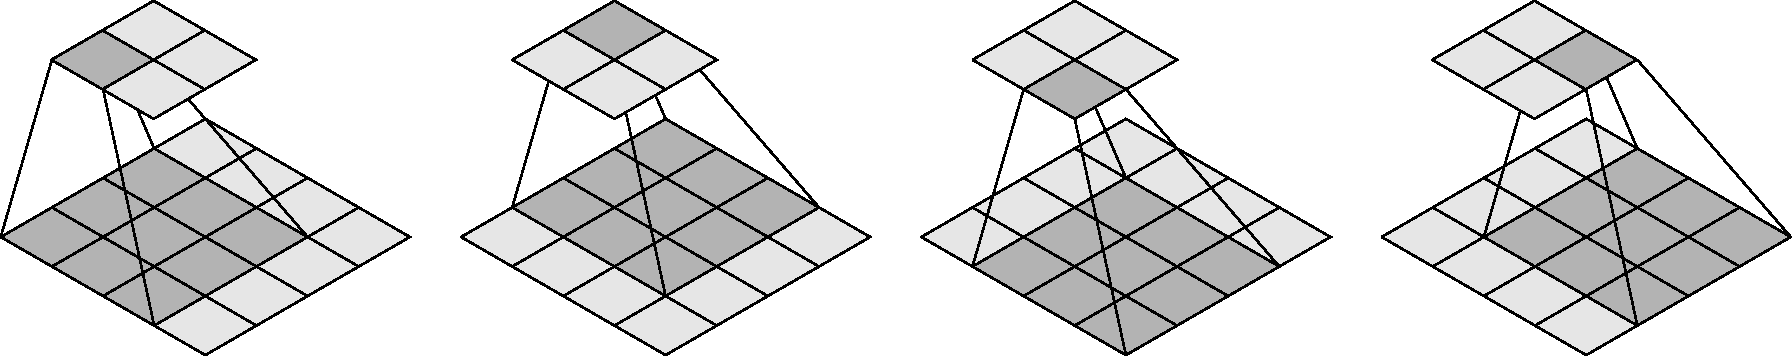
\includegraphics[width=\textwidth]{figures/cnn}
	\caption{
		CNN. Some more description.
	}
	\label{fig:cnn}
\end{figure}
%


\subsection{Table}
\label{sec:methodology:example:table}
%
Table \ref{tab:example-table} has two columns and three rows.

\begin{table}[h]
	\centering
	\begin{tabular}{rl}
		\toprule
		Column 1 & Column 2 \\
		\midrule
		1        & A        \\
		2        & B        \\
		3        & C        \\
		\bottomrule
	\end{tabular}
	\caption{Table. Detailed description.}
	\label{tab:example-table}
\end{table}


\subsection{Math}
\label{sec:methodology:example:math}
%
Equations \ref{eq:precision} and \ref{eq:recall} are important.
%
\begin{equation}
	precision = \frac{TP}{TP + FP}
	\label{eq:precision}
\end{equation}
%
\begin{equation}
	recall = \frac{TP}{TP + FN}
	\label{eq:recall}
\end{equation}
%


\subsection{Citation}
\label{sec:methodology:example:citation}
%
Some references about data imputation~\cite{jagerBenchmarkDataImputation2021}, the GreenDB~\cite{jagerGreenDBDatasetBenchmark2022, jagerGreenDBProductbyProductSustainability2022, gossenNudgingSustainableConsumption2022}, or how to scale \glspl{NN}~\cite{jagerParallelizedTrainingDeep2018}.


\subsection{Footnote}
\label{sec:methodology:example:footnote}
%
Footnotes can be used to add additional information\footnote{Additional information about XYZ.} or links\footnote{\url{calgo-lab.de}}.


\section{Summary}
\label{sec:methodology:summary}

It can be helpful to summarize what is written here.
%% LaTeX2e class for student theses
%% conclusion.tex
%%
%% Berlin University of Applied Sciences and Technology
%% Fachbereich 6: Informatik und Medien
%% Cognitive Algorithms Lab (Calgo Lab)
%%
%% Prof. Dr. Felix Bießmann
%% felix.biessmann@bht-berlin.de
%%
%% Version 0.1, 2023-03-26
%%
%% -----------------------------------------------------


\chapter{Conclusion and Future Work}
\label{ch:conclusion_future_work}

Lorem Ipsum


\section{Conclusion}
\label{sec:conclustion}

Lorem Ipsum

\paragraph{Limitations} Lorem Ipsum




\section{Future Work}
\label{sec:future_work}

\paragraph{Paragraph 1} Lorem Ipsum

\paragraph{Paragraph 2} Lorem Ipsum

\paragraph{Paragraph ...} Lorem Ipsum







%% -----------------
%% |  Bibliography |
%% -----------------

%% Add entry to the table of contents for the bibliography

\printbibliography[heading=bibintoc]


%% --------------
%% |   Appendix   |
%% --------------
% Optional
\appendix
%% LaTeX2e class for student theses
%% appendix.tex
%%
%% Berlin University of Applied Sciences and Technology
%% Fachbereich 6: Informatik und Medien
%% Cognitive Algorithms Lab (Calgo Lab)
%%
%% Prof. Dr. Felix Bießmann
%% felix.biessmann@bht-berlin.de
%%
%% Version 0.1, 2023-03-26
%%
%% -----------------------------------------------------

\chapter{Results}
\label{appendix:results}
%
Here, it could make sense to add all experiment results or pseudo code.


\section{Experiment 1}
\label{appendix:results:experiment_1}
%
Lorem Ipsum

\end{document}
